\documentclass[11pt]{article}

% ==== PACKAGES ==== %
% \usepackage{fullpage}
\usepackage{amsmath,amssymb,amsthm}
\usepackage{epic}
\usepackage{eepic}
\usepackage{hyperref}
\usepackage{listings}
\usepackage{float}
\usepackage{graphicx}
\usepackage{fancyhdr}
\usepackage{color}
\usepackage{bbm}
\usepackage[letterpaper, margin=1in]{geometry}

% ==== MARGINS ==== %
% \pagestyle{empty}
% \setlength{\oddsidemargin}{0in}
% \setlength{\textwidth}{6.8in}
% \setlength{\textheight}{9.5in}

\pagestyle{fancy}
\fancyhf{}
\rhead{ASEN 5044}
\lhead{Homework 1}
\rfoot{Page \thepage}


\newtheorem*{solution*}{Solution}
\newtheorem{lemma}{Lemma}[section]
\newtheorem{theorem}[lemma]{Theorem}
\newtheorem{claim}[lemma]{Claim}
\newtheorem{definition}[lemma]{Definition}
\newtheorem{corollary}[lemma]{Corollary}
\lstset{moredelim=[is][\bfseries]{[*}{*]}}

% ==== DOCUMENT PROPER ==== %
\begin{document}

\thispagestyle{empty}

% --- Header Box --- %
\newlength{\boxlength}\setlength{\boxlength}{\textwidth}
\addtolength{\boxlength}{-4mm}

\begin{center}\framebox{\parbox{\boxlength}{\bf
      Statistical Estimation \hfill Homework 2\\
      ASEN 5044 Fall 2018 \hfill Due Date: Sep 20, 2018\\
      Name: Andrew Kramer \hfill PhD Student
}}
\end{center}

\section*{Exercise 1}
Consider the 2-mass/3-spring system presented in lecture 4, where the continuous time state definition and inputs are the same, but the observed sensor inputs are now given by 
\begin{equation*}
	y(t) = \begin{bmatrix} 1 & 0 & 0 & 0 \\ 0 & 1 & 0 & -1 \end{bmatrix}x(t) + \begin{bmatrix} 0 & 0 \\ 0 & 0 \end{bmatrix} u(t)
\end{equation*}

\subsection*{Problem (a)}
Find the discrete time LTI representation for this system using a step size of $\Delta T = 0.05$ sec. How does this sampling rate compare with the system's Nyquist limit?

\subparagraph*{}
Recalling lecture 4, the state of the system is given by $x(t) = [q_1(t),\ \dot{q}_1(t),\ q_2(t),\ \dot{q}_2(t)]^T$ where $q_i$ is the displacement of mass $i$ and $u(t) = [u_1(t),\ u_2(t)]^T$ where $u_1$ is the force between the two masses and $u_2$ is the force on mass 2. The CT LTI system model is given by $\dot{x} = Ax(t)+bu(t)$ where
\begin{align*}
	A &= \begin{bmatrix} 0&1.0&0&0 \\ -2.0&0&1.0&0 \\ 0&0&0&1.0 \\ 1.0&0&-2.0&0 \end{bmatrix} \\ 
	B&= \begin{bmatrix} 0&0 \\ -1&0 \\ 0&0 \\ 1&1 \end{bmatrix}
\end{align*}
This is relatively simple to convert to a discrete time system. We only need to find $e^{\hat{A}\Delta t}$ where
\begin{equation*}
	\hat{A} = \begin{bmatrix} 0&1&0&0&0&0 \\ -2&0&1&0&-1&0 \\ 0&0&0&1&0&0 \\ 1&0&-2&0&1&1 \\ 0&0&0&0&0&0 \\ 0&0&0&0&0&0 \end{bmatrix} 
\end{equation*}
The discretized system is described by $x(k+1)=Fx(k)+Gu(k)$ where $F$ is the upper left $4\times 4$ block of $e^{\hat{A}\Delta t}$ and $G$ is the upper right $4\times 2$ block:
\begin{align*}
	F&=\begin{bmatrix}1.0 & 0.05 & 0.001 & 0.0 \\ -0.1 & 1.0 & 0.05 & 0.001 \\ 0.001 & 0.0 & 1.0 & 0.05 \\ 0.05 & 0.001 & -0.1 & 1.0 \end{bmatrix} \\
	G&=\begin{bmatrix} -0.001 & 0.0 \\ -0.05 & 0.0 \\ 0.001 & 0.001 \\ 0.05 & 0.05 \end{bmatrix}
\end{align*}
To satisfy the Nyquist sampling criterion for this system the following inequality must hold $\frac{\pi}{\Delta t} > 2|\lambda_\text{max}|$ where $|\lambda_\text{max}|$ is the largest complex magnitude among all the eigenvalues of $A$. In this case that magnitude is $1.732$. 
\begin{align*}
	\frac{\pi}{\Delta t} &= 62.83 \\
	2|\lambda_\text{max}| &= 3.464
\end{align*}
Clearly in this case the sampling frequency is well within the Nyquist limit for this system.

\subsection*{Problem (b)}
Show that the DT system is observable.

\subparagraph*{}
We'll start by building candidates for our observability matrix $\mathbb{O}$ and checking if they are full rank. The simplest possible case, $\mathbb{O} = H$ is rank deficient, because column $4$ of $H$ is simply column $2$ multiplied by $-1$.
\begin{equation*}
	H = \begin{bmatrix} 1 & 0 & 0 & 0 \\ 0 & 1 & 0 & -1 \end{bmatrix}
\end{equation*}
The next possibility, $[H,\ HF]^T$, is full rank. 
\begin{equation*}
	\mathbb{O} = \begin{bmatrix} H \\ HF \end{bmatrix} = \begin{bmatrix} 1.0 & 0.0 & 0.0 & 0.0 \\ 0.0 & 1.0 & 0.0 & -1.0 \\ 1.0 & 0.05 & 0.001 & 0.0 \\ -0.15 & 1.0 & 0.15 & -1.0 \end{bmatrix}
\end{equation*}
This means the system is fully observable from two observations. This makes physical sense, as the displacement of mass 1, $x_1$ is directly measurable (as $y_1$) so we should be able to find the velocity of mass 1, $x_2$ with two measurements of its position. Then, if we know velocity of mass 1 and the relative velocity of the two masses, $y_2$ it is possible to calculate the velocity of mass 2, $x_4$. Lastly, knowing the velocity of mass 2 over one timestep will also allow us to calculate its displacement $x_3$ over that timestep.

\subsection*{Problem (c)}
Suppose the system starts from some unknown initial condition $x(0)$ at $k=0$ and is stimulated by an external set of ZOH inputs $u$ at the $\Delta T = 0.05$ sec sampling rate from $t=0$ to $t=5$ seconds, where $u(t)=[\sin(t), 0.1\cos(t)]^T$, and the resulting output $y(k)$ at each sampling instant from $t=0.05$ sec ($k=1$) to $t=5$ sec is recorded in \texttt{hw3problemdata.mat}. Derive a linear system of equations in matrix-vector form that would allow you to estimate the unknown initial condition $x(k=0)$ using all the available logged $y$ and $u$ data.

\subparagraph*{}
We can regress $x(0)$ from the logged $n$ measurements by stacking the measurements to form an $np\times1$ column vector $Y$ which will follow the relationship
\begin{equation*}
	Y = \mathbb{O}x(0)
\end{equation*}
where $\mathbb{O}=[HF^0,\ HF^1,\ HF^2,\ \dots, HF^{n-1}]^T$. However, this only applies when there is no input $u(t)$. If the input is nonzero our relationship becomes more complicated:
\begin{align*}
	y(0) &= Hx(0) \\
	y(1) = Hx(1) &= H(Fx(0) + Gu(0)) \\
	y(2) = Hx(2) = H(Fx(1) + Gu(1)) &= H(F(Fx(0) + Gu(0)) + Gu(1)) \\
	&= HF^2x(0) + HFGu(0) + Gu(1) \\
	y(n-1) &= HF^{n-2}x(0) + \sum_{i=0}^{n-1}HF^{n-2-i}Gu(i)
\end{align*}
So our equation for the measurements $Y$ becomes
\begin{equation*}
	Y = \mathbb{O}x(0) + U
\end{equation*}
where
\begin{equation*}
	U=\begin{bmatrix} 0 \\ HGu(0) \\ HFGu(0) + HGu(1) \\ \dots \\ \sum_{i=0}^{n-2}HF^{n-2-i}Gu(i) \end{bmatrix}
\end{equation*}
We can still solve for $x(0)$ similar to the method used when $u(t)=0$:
\begin{equation*}
	x(0) = (\mathbb{O}^T\mathbb{O})^{-1}\mathbb{O}^T(Y-U)
\end{equation*}

\subsection*{Problem (d)}
Estimate $x(k=0)$ and plot all the remaining states $x(k)$ for $k\geq 1$ vs time (in seconds) and separately plot their corresponding 'predicted' outputs $y(k)$ vs. time for all $k\geq 1$ in the recorded output time series. Validate your estimate by also separately plotting the differences between the 'predicted' and recorded $y(k)$ values vs. time.

\subparagraph*{}
In solving $(\mathbb{O}^T\mathbb{O})^{-1}\mathbb{O}^TY$ we find that $x(0)=[0.114,\ 0.272,\ -0.423,\ -0.814]$. See figure \ref{fig:1d_states} below for a plot of the predicted states vs. time and figure \ref{fig:1d_meas} for the predicted outputs. Figure \ref{fig:1d_diffs} shows the difference between the predicted and actual measurements. The predicted measurements match the actual measurements exactly in frequency, though their amplitude differs.

\begin{figure}[h!]
	\centering
	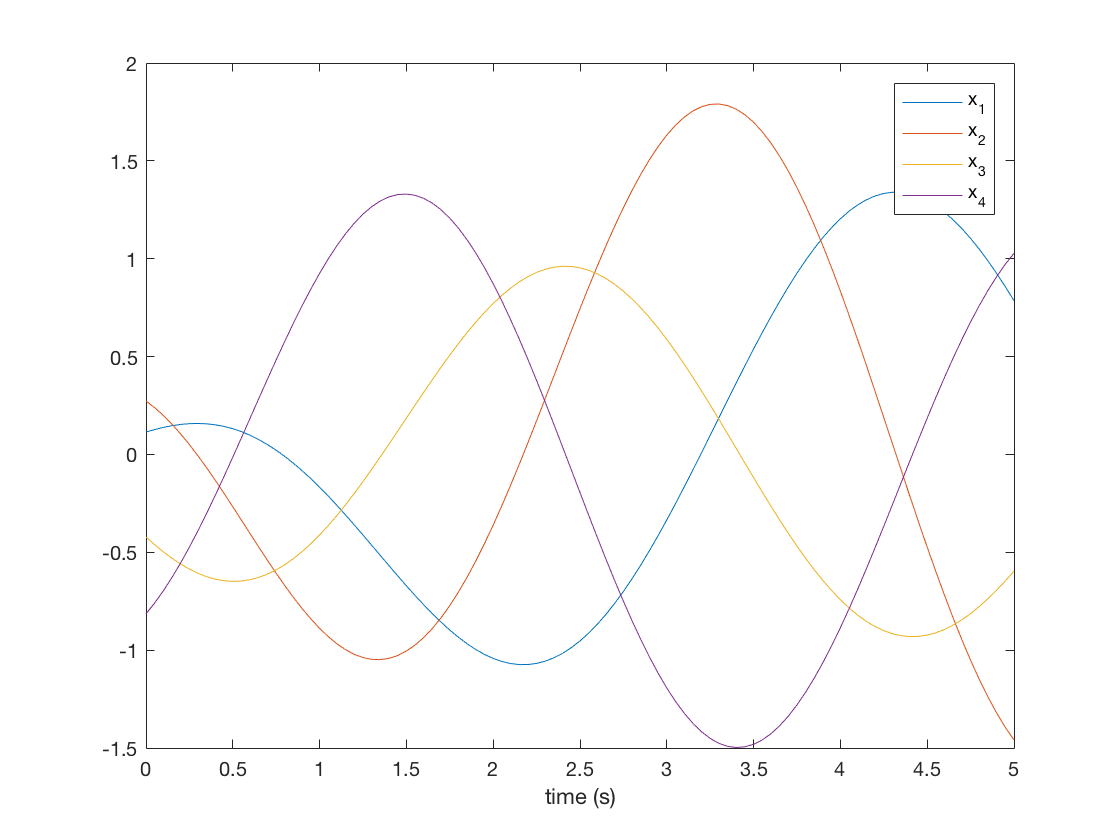
\includegraphics[width=0.6\linewidth]{1d_state_plot.png}
	\caption{predicted states}
	\label{fig:1d_states}
\end{figure}
\begin{figure}[h!]
	\centering
	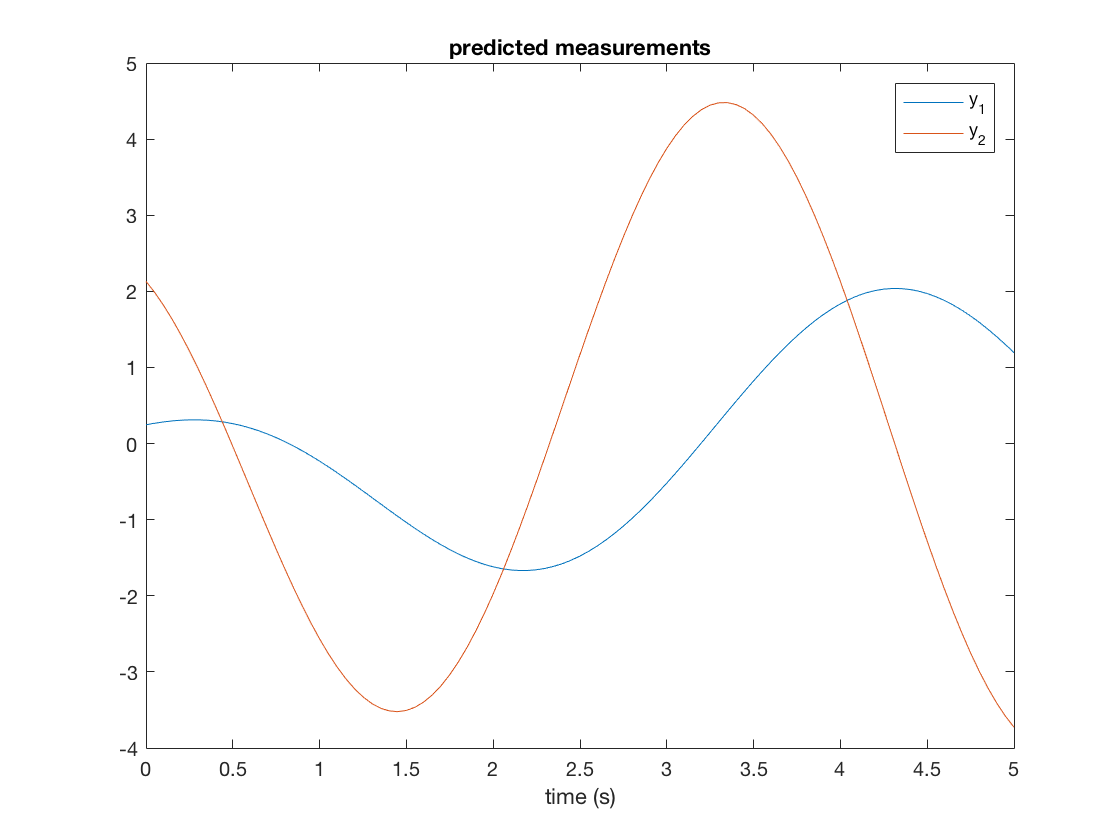
\includegraphics[width=0.6\linewidth]{1d_pred_meas.png}
	\caption{predicted measurements}
	\label{fig:1d_meas}
\end{figure}
\begin{figure}[h!]
	\centering
	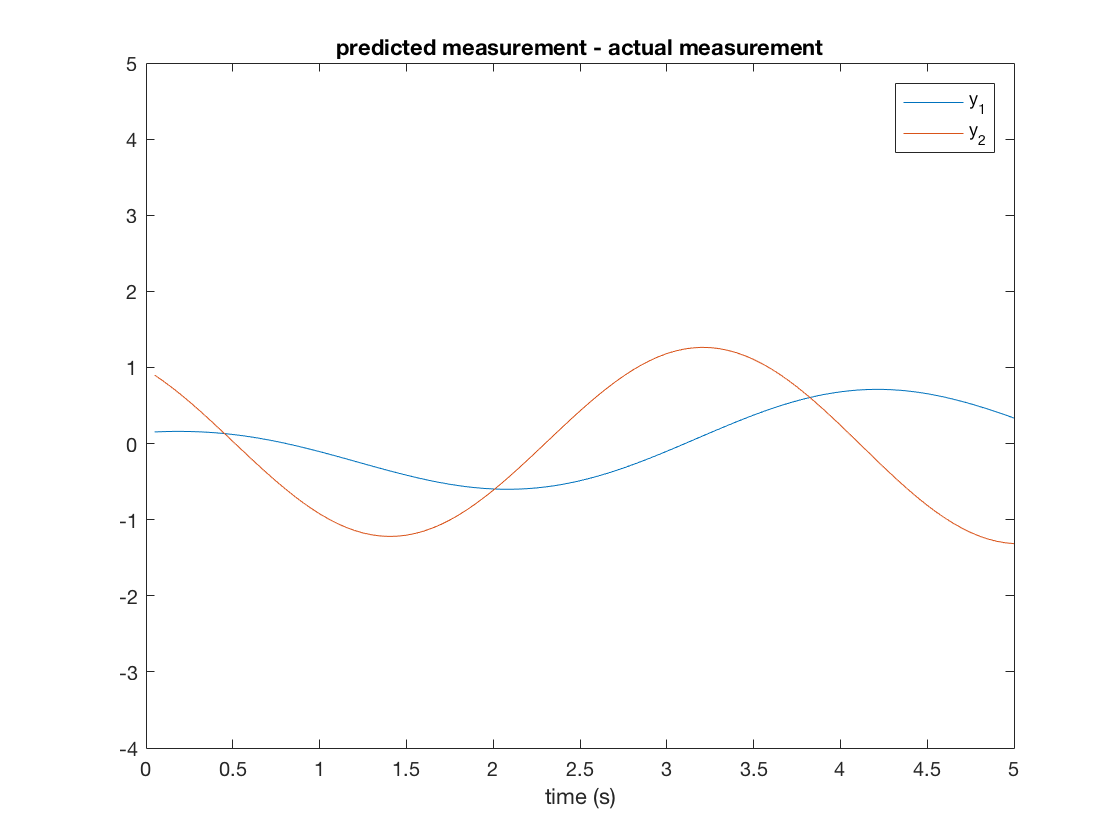
\includegraphics[width=0.6\linewidth]{1d_meas_diffs.png}
	\caption{difference between predicted and actual measurements}
	\label{fig:1d_diffs}
\end{figure}

\subsection*{Problem (e)}
How many vector measurements $y(k)$ are actually needed to estimate $x(0)$, i.e. do you need to use all available measurements, or some smaller number? Is this consistent with an analysis of the observability matrix $\mathbb{O}$ and Grammian $\mathbb{O}^T\mathbb{O}$? Explain how and why the required number of vector measurements would theoretically change if the $y(k)$ data were instead given by three different position sensors for the first mass, where 
\begin{equation*}
	H=\begin{bmatrix} 1&0&0&0 \\ 1&0&0&0 \\ 1&0&0&0 \end{bmatrix}
\end{equation*}

\subparagraph*{}
Because the observability matrix is full rank when only 2 measurements are used (i.e. $\text{rank}([H,\ HF]^T)=4$), we only need 2 measurements to estimate $x(0)$. If $H$ were instead given by three different position sensors on the first mass, the system would require 4 measurements to be observable. This is because every entry in column $i$ of $HF^k$ will be equal to the first entry in column $i$ of $F^k$ for every possible value of $k$. This means $\text{rank}(\mathbb{O})=1$ when $\mathbb{O}=H$, $\text{rank}(\mathbb{O})=2$ when $\mathbb{O}=[H,\ HF]^T$, $\text{rank}(\mathbb{O})=3$ when $\mathbb{O}=[H,\ HF,\ HF^2]^T$ and $\mathbb{O}$ is full rank when $\mathbb{O}=[H,\ HF,\ HF^2,\ HF^3]^T$.

\subsection*{Problem (f)}
What happens to the observability of the system if only the first row of the output $y(k)$ is used for all $k\geq 1$? What if only the second row of the output vector $y(k)$ is used instead? Provide a physical explanation in each case.

\subparagraph*{}
When only the first row of $y(k)$ is used the system is observable when 4 measurements are used. This case is the same as the one in part (e). If only the position of the first mass is known, then 4 measurements are required to be able to calculate the position, mass, and acceleration of the first mass over 2 timesteps. If the acceleration of the mass 1 is known then we also know the net force on that mass. Because the position of mass 1 is also known we know the force from spring 1. From these two quantities, we can calculate the force from (and hence the displacement of) spring 2. Because we know the position of mass 1 and displacement of spring 2 we can calculate the position of mass 2. This only used 3 measurements, however. We need the 4th measurement because we also need to calculate the velocity of mass 2. To do this we need to calculate its position at 2 timesteps, hence the need for the 4th measurement. \\
If only the second row of $y(k)$ is used the system is never observable. This is because for all $n>1$ $\mathbb{O}_3=-\mathbb{O}$ and $\mathbb{O}_4=-\mathbb{O}_2$ where $\mathbb{O}_i$ denotes the $i^\text{th}$ column of $\mathbb{O}$. This means $\text{rank}(\mathbb{O})=2$ for $n>1$. The state of this system is never observable because we only ever get information about the relative velocity of the 2 masses. We could integrate two relative velocity measurements to get their relative displacement. However, to get the full state we need the absolute displacements of the masses. To get the absolute displacements of the masses at timestep $k$ we would need to know their absolute displacements at some other timestep, and we will never get this information using only the second row of $y(k)$.

\section*{Exercise 2}
(Luenberger, 1979) discusses a simple model for the national income dynamics. The national income $y_k$ in year $k$ in terms of consumer expenditure $c_k$, private investment $i_k$ and government expenditure $g_k$ is assumed to be given by $y_k=c_k+i_k+g_k$, where the interrelations between these quantities are specified by $c_{k+1}=\alpha y_k$ and $i_{k+1}=\beta(c_{k+1}-c_k)$. The constant $\alpha$ is called the marginal propensity to consume, while $\beta$ is a growth coefficient. Typically, $0<\alpha<1$ and $\beta > 0$.

\subsection*{Problem (a)}
Show that these relations can be rearranged into the following discrete time state space model with ($F,G,H,M$) matrix parameters:
\begin{align*}
	x_{k+1} = \begin{bmatrix} x_{1,k+1} \\ x_{2,k+1} \end{bmatrix} &= \begin{bmatrix} \alpha & \alpha \\ \beta(\alpha-1) & \beta\alpha \end{bmatrix} \begin{bmatrix} x_{1,k} \\ x_{2,k} \end{bmatrix} + \begin{bmatrix} \alpha \\ \beta\alpha \end{bmatrix} u_k \\
	y_k &= \begin{bmatrix} 1 & 1 \end{bmatrix} \begin{bmatrix} x_{1,k} \\ x_{2,k} \end{bmatrix} + u_k
\end{align*}
where $x_{1,k}\equiv c_k$, $x_{2,k} \equiv i_k$, $u_k \equiv g_k$.

\subparagraph*{}
It is fairly simple to translate the formula for $y_k$ to matrix form:
\begin{align*}
	y_k &= c_k + i_k + g_k \\
	&= x_{1,k} + x_{2,k} + u_k \\
	&= \begin{bmatrix} 1 & 1 \end{bmatrix} \begin{bmatrix} x_{1,k} \\ x_{2,k} \end{bmatrix} + u_k \\
\end{align*}
Translating the formulas for $x_{1,k+1}$ and $x_{2,k+1}$ goes as follows:
\begin{align*}
	c_{k+1} = x_{1,k+1} &= \alpha y_k \\
	&= \alpha(c_k + i_k + g_k) \\
	&= \alpha(x_{1,k} + x_{2,k} + u_k) \\
	&= \alpha x_{1,k} + \alpha x_{2,k} + \alpha u_k \\
	\\
	i_{k+1} = x_{2,k+1} &= \beta(c_{k+1} - c_k) \\
	&= \beta(x_{1,k+1}-x_{1,k}) \\
	&= \beta(\alpha(x_{1,k} + x_{2,k} + u_k) - x_{1,k}) \\
	&= \beta(\alpha-1)x_{1,k} + \beta\alpha x_{2,k} + \beta\alpha u_k \\
	\\
	x_{k+1} &= \begin{bmatrix} \alpha & \alpha \\ \beta(\alpha-1) & \beta\alpha \end{bmatrix}\begin{bmatrix} x_{1,k} \\ x_{2,k} \end{bmatrix} + \begin{bmatrix} \alpha \\ \beta\alpha \end{bmatrix} u_k 
\end{align*}

\subsection*{Problem (b)}
Let the parameters $(\alpha,\beta)$ take on the following pairs of values: $(0.75,1),\ (0.75,1.5)$, and $(1.25,1)$. For each case determine the eigenvalues for the $F$ matrix, and also plot the states for $0\leq k\leq30$ when $u_k$ is a unit step input (i.e. $u_k=1$ for all $k>0$) and $x_0=[0,0]^T$. Comment on the stability and observability of the system in each case.

\subparagraph*{}
For the first pair of values, $(0.75,1.0)$, the eigenvalues of $F$ are $0.75\pm0.433j$ As the complex magnitudes of these eigenvalues are less than one, the eigenvalues of $F$ lie inside the unit circle. This means that the system is asymptotically stable for the given parameter values. Additionally, the observability matrix is full rank for $n=2$, 
\begin{equation*}
	\mathbb{O} = \begin{bmatrix} H \\ HF \end{bmatrix} = \begin{bmatrix} 1.0 & 1.0 \\ 0.5 & 1.5 \end{bmatrix}
\end{equation*}
so the system is observable from two measurements. See figure \ref{fig:2b_plot1} for a plot of the system states for $0\leq k\leq 30$.

\begin{figure}[h!]
	\centering
	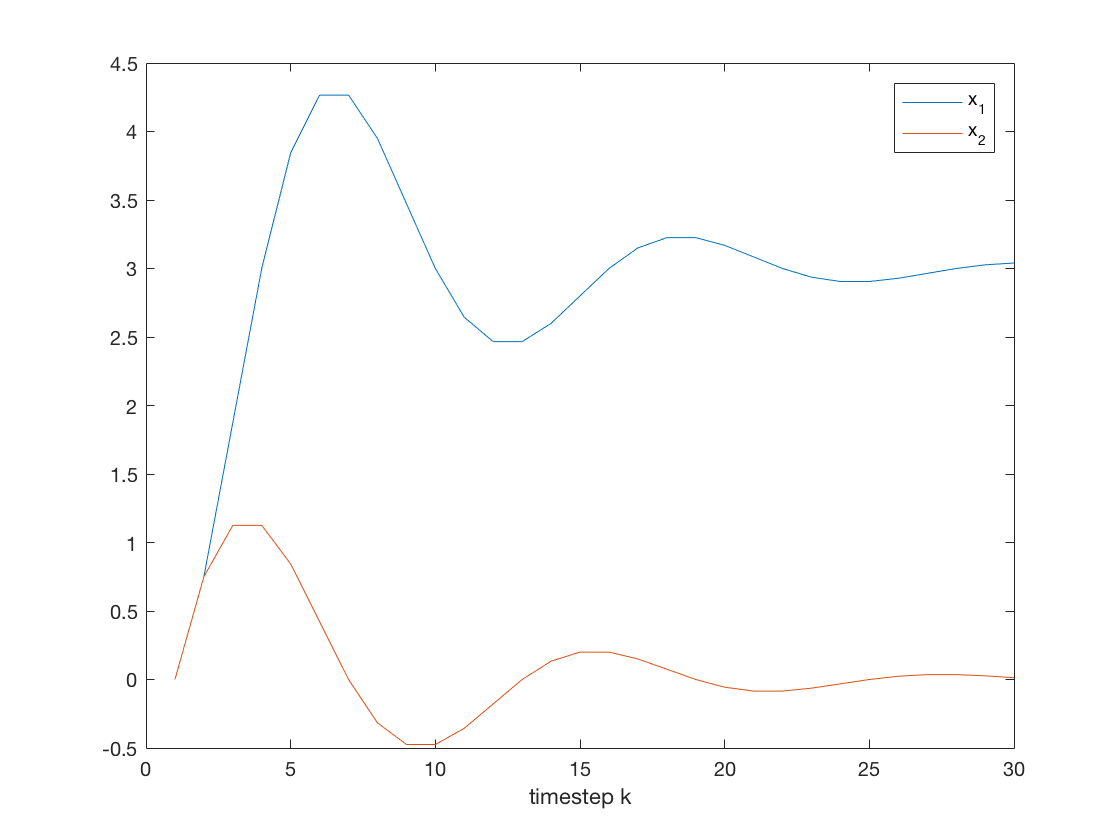
\includegraphics[width=0.6\linewidth]{2b_plot1.png}
	\caption{predicted states}
	\label{fig:2b_plot1}
\end{figure}

For the second pair of values, $(0.75,1.5)$, the eigenvalues of $F$ are $0.938\pm0.496j$ As the complex magnitudes of these eigenvalues are greater than one, the eigenvalues of $F$ lie outside the unit circle. This means that the system is asymptotically unstable for the given parameter values. Additionally, the observability matrix is full rank for $n=2$, 
\begin{equation*}
	\mathbb{O} = \begin{bmatrix} H \\ HF \end{bmatrix} = \begin{bmatrix} 1.0 & 1.0 \\ 0.375 & 1.875 \end{bmatrix}
\end{equation*}
so the system is observable from two measurements. See figure \ref{fig:2b_plot2} for a plot of the system states for $0\leq k\leq 30$.

\begin{figure}[h!]
	\centering
	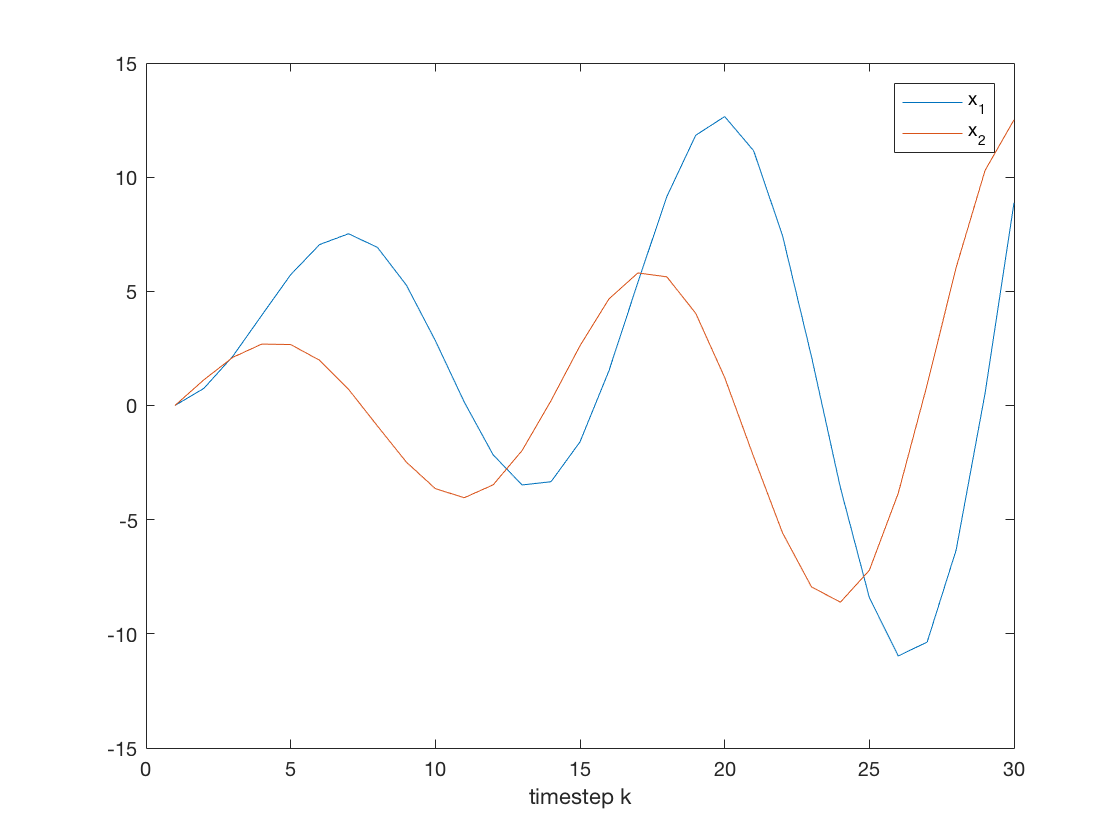
\includegraphics[width=0.6\linewidth]{2b_plot2.png}
	\caption{predicted states}
	\label{fig:2b_plot2}
\end{figure}

For the last pair of values, $(1.25,1.0)$, the eigenvalues of $F$ are $1.809$ and $0.691$. As the complex magnitudes of one of these eigenvalues is not less than one, that eigenvalue of $F$ lies outside the unit circle. This means that the system is asymptotically unstable for the given parameter values. Additionally, the observability matrix is full rank for $n=2$, 
\begin{equation*}
	\mathbb{O} = \begin{bmatrix} H \\ HF \end{bmatrix} = \begin{bmatrix} 1.0 & 1.0 \\ 1.5 & 2.5 \end{bmatrix}
\end{equation*}
so the system is observable from two measurements. See figure \ref{fig:2b_plot3} for a plot of the system states for $0\leq k\leq 30$.

\begin{figure}[h!]
	\centering
	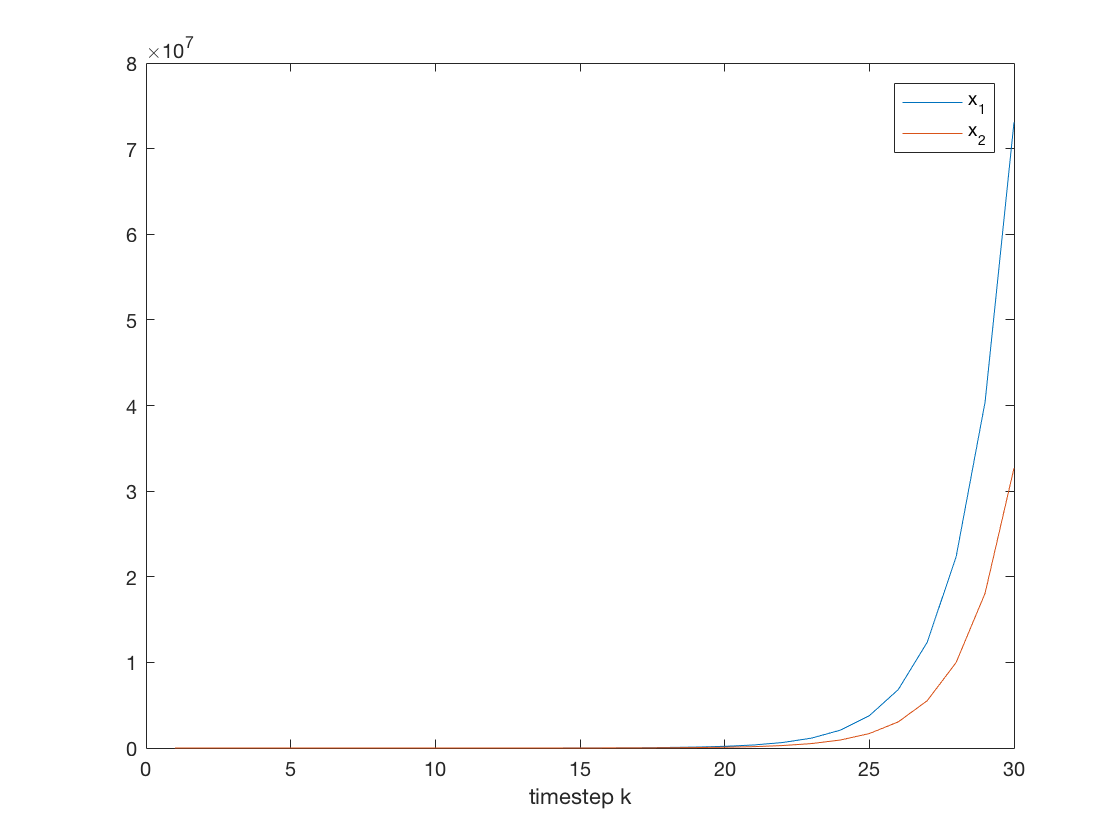
\includegraphics[width=0.6\linewidth]{2b_plot3.png}
	\caption{predicted states}
	\label{fig:2b_plot3}
\end{figure}

\subsection*{Problem (c)}
For each of the parameter cases in (b), plot the states for $k\geq0$ when $u_k=0$ for all time $k$ and $x_0=[5,1]^T$. Comment on your results.

\subparagraph*{}
Figure \ref{fig:2c_plot1}, below, shows the state behavior when $\alpha=0.75$ and $\beta=1$. Notice the system is still stable, but it converges to a different values than when $u(k)$ is nonzero.

\begin{figure}[h!]
	\centering
	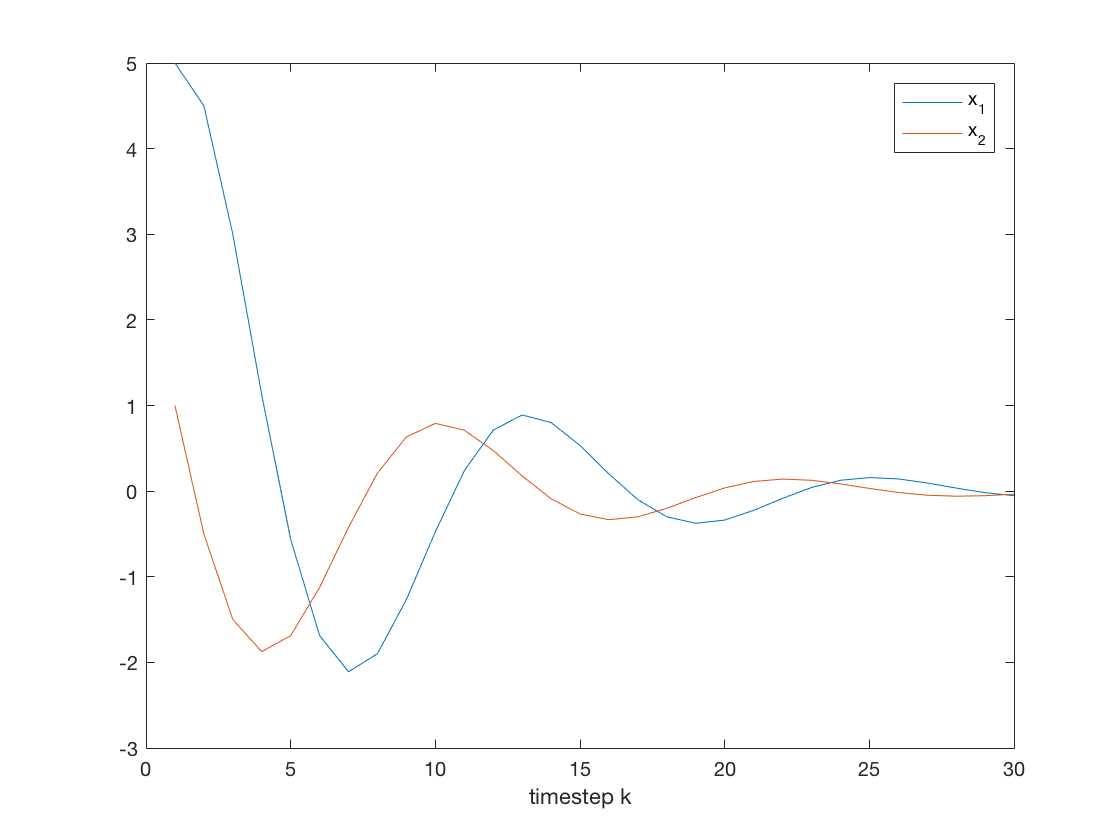
\includegraphics[width=0.6\linewidth]{2c_plot1.png}
	\caption{predicted states}
	\label{fig:2c_plot1}
\end{figure}

Figure \ref{fig:2c_plot2}, below, shows the state behavior when $\alpha=0.75$ and $\beta=1.5$. The system is still asymptotically unstable.

\begin{figure}[h!]
	\centering
	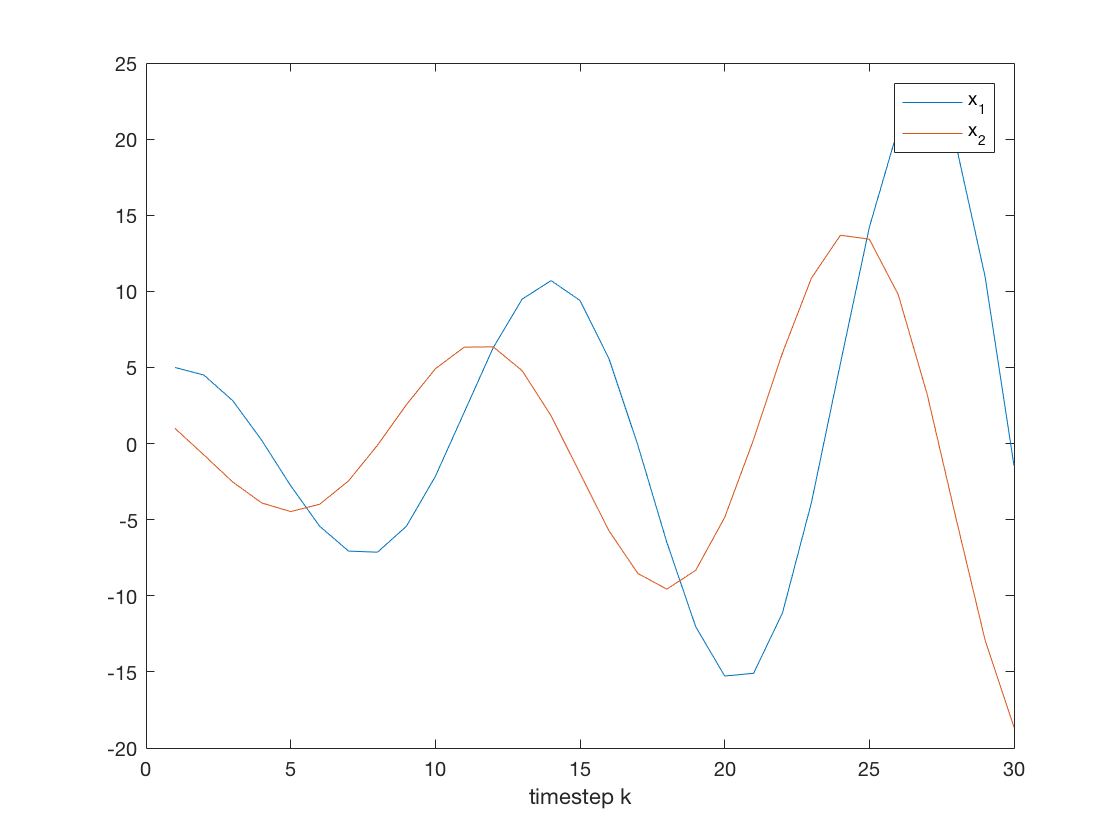
\includegraphics[width=0.6\linewidth]{2c_plot2.png}
	\caption{predicted states}
	\label{fig:2c_plot2}
\end{figure}

Figure \ref{fig:2c_plot1}, below, shows the state behavior when $\alpha=1.25$ and $\beta=1$. The system is still asymptotically unstable.

\begin{figure}[h!]
	\centering
	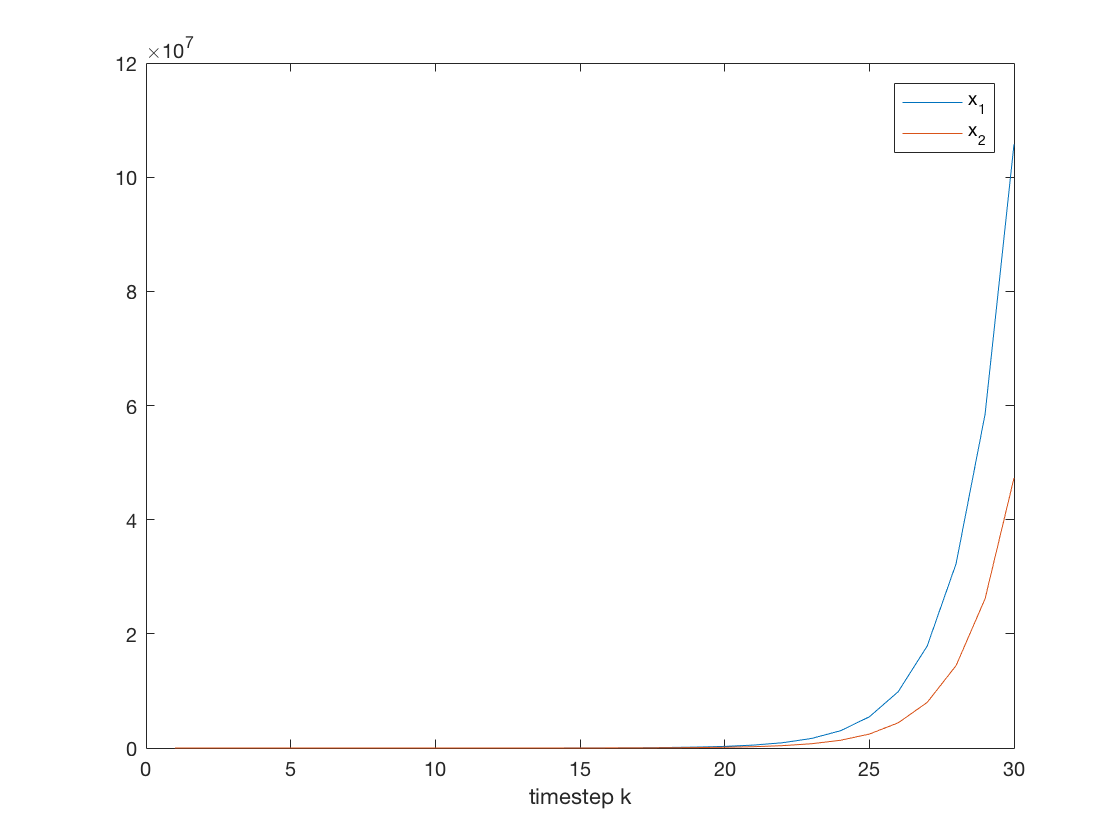
\includegraphics[width=0.6\linewidth]{2c_plot3.png}
	\caption{predicted states}
	\label{fig:2c_plot3}
\end{figure}

\subsection*{Problem (d)}
For each of the parameter cases in (c), simulate a sequence of observations $y(0),\dots,y(9)$ and use all the data to estimate the initial condition $x_0$ as if it were unknown (assume $u_k$ is the same as in case (c)). Show a plot of your observation sequence vs time, and report your resulting estimates in each case (be sure to explain the approach used to get the estimates, and validate your estimates by plotting the resulting predicted $y(k)$ outputs vs time against the real $y(k)$ data generated in each case).

\subparagraph*{}
Figure \ref{fig:2d_plot1}, below shows the predicted measurements for $\alpha=0.75$ and $\beta=1$. The predicted initial condition for this system was $x_0=[5,1]^T$, which perfectly matches the actual initial condition. The predicted initial condition was obtained by multiplying the grammian of the $30\times2$ observability matrix with the measurements plotted below as in $x(0)=(\mathbb{O}^T\mathbb{O})^{-1}\mathbb{O}Y$. 

\begin{figure}[h!]
	\centering
	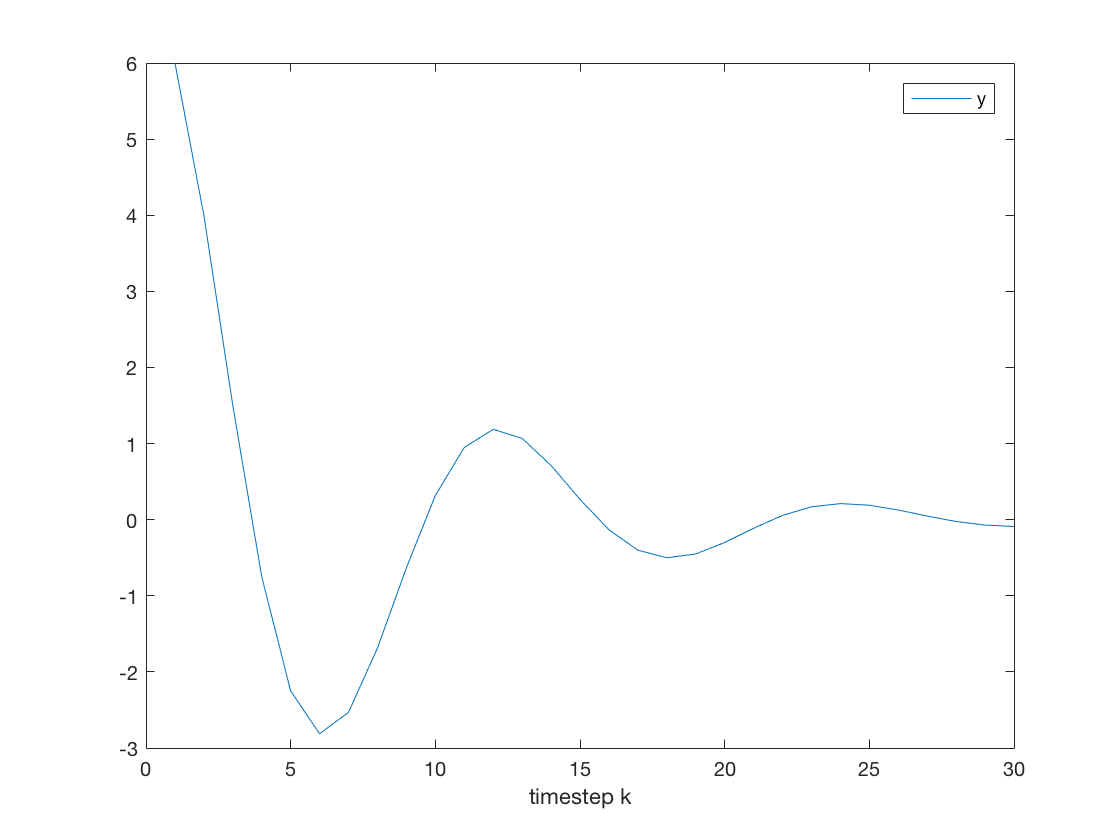
\includegraphics[width=0.6\linewidth]{2d_plot1.png}
	\caption{predicted measurements}
	\label{fig:2d_plot1}
\end{figure}

Figure \ref{fig:2d_plot2}, below shows the predicted measurements for $\alpha=0.75$ and $\beta=1.5$. The predicted initial condition for this system was $x_0=[5,1]^T$, which perfectly matches the actual initial condition. The predicted initial condition was obtained by multiplying the grammian of the $30\times2$ observability matrix with the measurements plotted below as in $x(0)=(\mathbb{O}^T\mathbb{O})^{-1}\mathbb{O}Y$. 

\begin{figure}[h!]
	\centering
	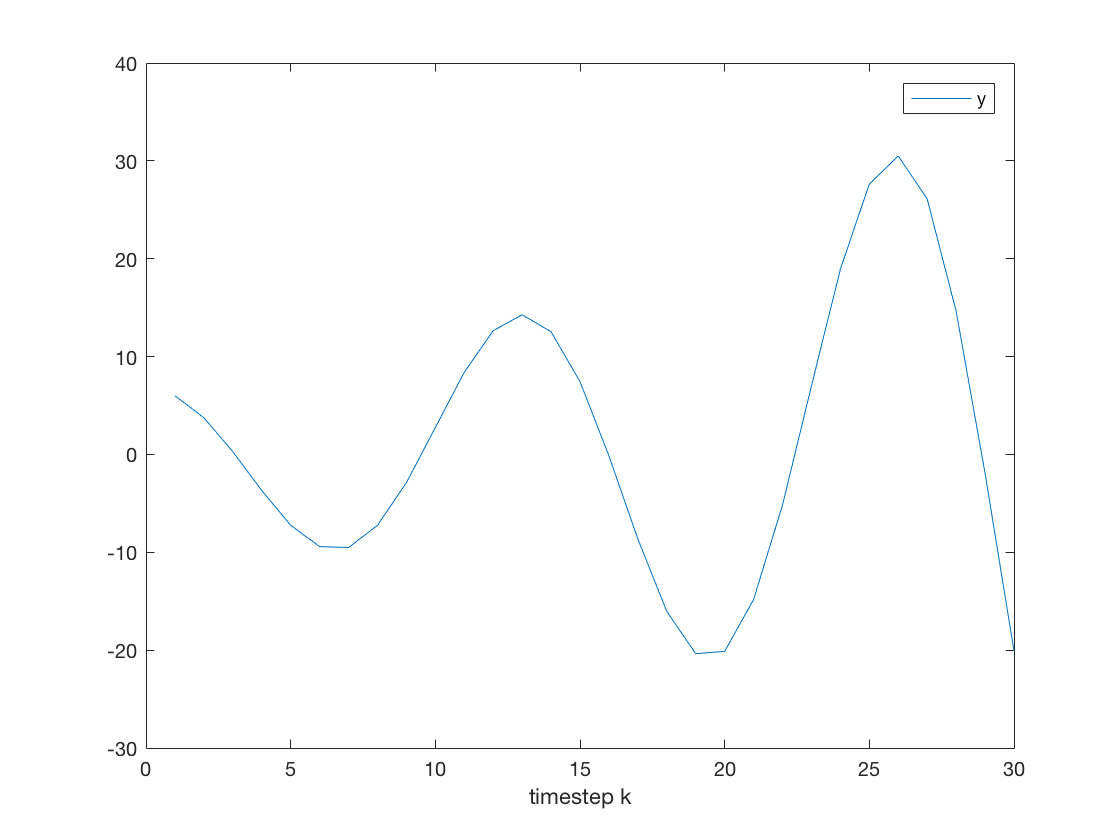
\includegraphics[width=0.6\linewidth]{2d_plot2.png}
	\caption{predicted measurements}
	\label{fig:2d_plot2}
\end{figure}

Figure \ref{fig:2d_plot3}, below shows the predicted measurements for $\alpha=1.25$ and $\beta=1$. The predicted initial condition for this system was $x_0=[4.72,1.12]^T$, which does not match the actual initial condition. The predicted initial condition was obtained by multiplying the grammian of the $30\times2$ observability matrix with the measurements plotted below as in $x(0)=(\mathbb{O}^T\mathbb{O})^{-1}\mathbb{O}Y$. The discrepancy between the actual and predicted $x_0$ could be explained by the fact that the system was so unstable the state values got high enough to cause numerical errors, which resulted in the grammian of the observability matrix being nearly singular. This caused an innacurate prediction of $x_0$. 

\begin{figure}[h!]
	\centering
	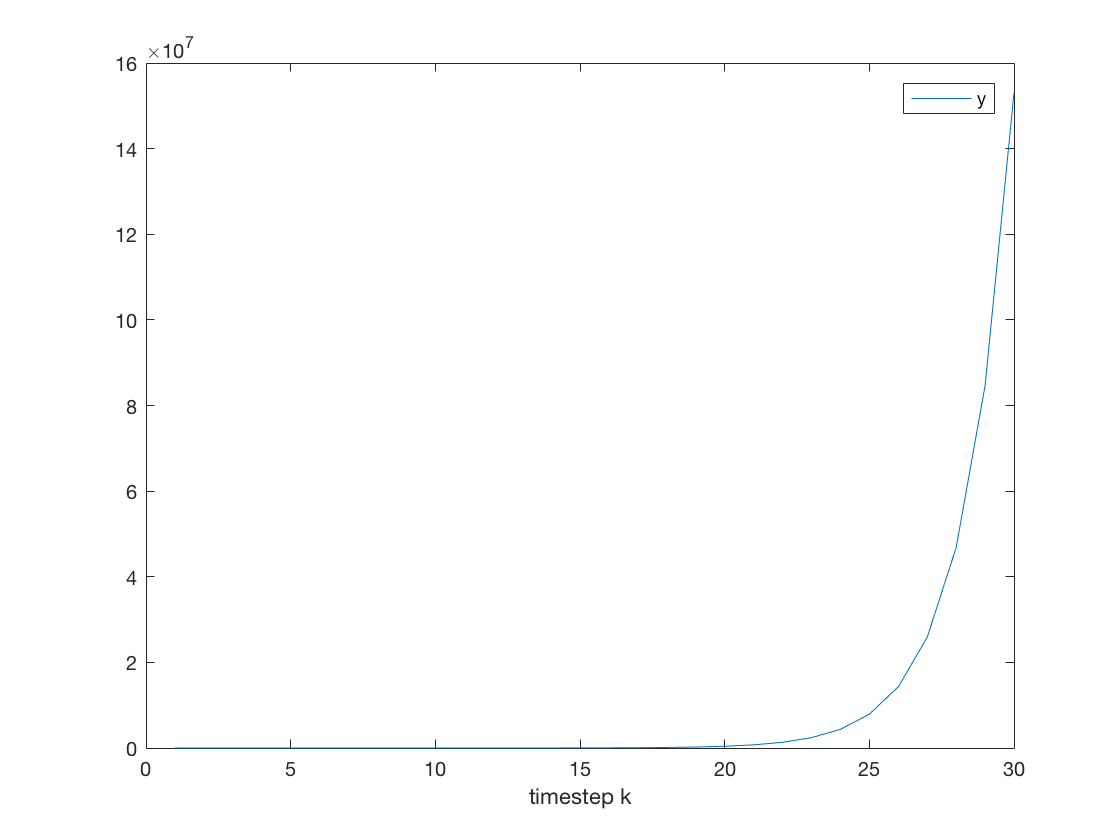
\includegraphics[width=0.6\linewidth]{2d_plot3.png}
	\caption{predicted measurements}
	\label{fig:2d_plot3}
\end{figure}

\section*{Exercise 3}
You are waiting around Gary Slick's dealership while your new Ferrari is being serviced when you notice local folk hero Pladimir Vutin walk in and start haggling with Slick over a vintage GAZ Chaika that is prominently on display. You can't help but overhear their discussion, and record the following discrete time series for Slick's offers ($z_1$, in tens of thousands of dollars) and Vutin's offers ($z_2$, in tens of thousands of dollars), stacked into the vector $z(k)=[z_1(k),z_2(k)]^T$,
\begin{align*}
	z(0) = \begin{bmatrix} 100 \\ 20 \end{bmatrix},\ z(1) &= \begin{bmatrix} 43.6658 \\ 39.2815 \end{bmatrix},\ z(2) = \begin{bmatrix} 40.5785 \\ 40.3382 \end{bmatrix} \\
	z(3) = \begin{bmatrix} 40.4093 \\ 40.3961 \end{bmatrix},\ z(4) &= \begin{bmatrix} 40.4 \\ 40.3993 \end{bmatrix},\ z(5) = \begin{bmatrix} 40.3995 \\ 40.3995 \end{bmatrix}
\end{align*}
Having conducted your own negotiation with Slick recently, you assume the dynamics of $z(k)$ could reasonably be modeled as
\begin{align*}
	z_1(k+1)&=z_1(k)+\lambda[z_1(k) - z_2(k)] \\
	z_2(k+1)&=z_2(k)+\mu[z_1(k)-z_2(k)]
\end{align*}
where the constants $\lambda$ and $\mu$ describe Slick's and Vutin's update parameters, respectively. You don't know what values of $\lambda$ and $\mu$ apply for this particular negotiation - but you'd sure like to figure out how Vutin galloped away with Slick's shirt on this deal.
\subsection*{Problem (a)}
Suppose the 'unknown state' to be estimated in this case is $x(k)=[\lambda,\mu]^T$, and (based on what you recorded) the 'observed output' for $k=0,1,2,\dots$ is taken to be $y(k+1)=[g(k+1),p(k+1)]^T$, where $g(k+1)=z_1(k+1)-z_1(k)$ and $p(k+1) = z_2(k+1)-z_2(k)$. Find a suitable DT linear state space system model for this problem, and discuss any interesting features of the $(F,G,H,M)$ matrix parameters for the model (e.g. which are time invariant or time varying?).

\subparagraph*{}
In the expression for $g(k+1)$ we can replace $z_1(k+1)$ with $z_1(k)+\lambda[z_1(k)-z_2(k)]$ which gives us $g(k+1) = \lambda[z_1(k)-z_2(k)]$. We can do an analagous operation for $p(k+1)$, giving us $y(k+1) = Hx$ where:
\begin{equation*}
	H=\begin{bmatrix} z_1(k)-z_2(k) & 0 \\ 0 & z_1(k)-z_2(k) \end{bmatrix}
\end{equation*}
In this case, the $H$ matrix is time varying. Getting the $F$ matrix is much simpler. Because the problem states that $\mu$ and $\lambda$ are constant, $x(k+1) = x(k)$. So the $F$ matrix is simply identity. There are no inputs to the system, so $G$ and $M$ are zero.

\subsection*{Problem (b)}
Under what conditions can the $\lambda$ and $\mu$ parameters be identified? Give a careful, precise mathematical justification and interpretation.

\subparagraph*{}
$\lambda$ and $\mu$ are observable from a single observation when $z_1(k) - z_2(k)\neq0$. In linear algebra terms, this is because the $H$ matrix is full rank only if $z_1(k)-z_2(k)\neq0$. If that is not the case, the $H$ matrix is a $2\times2$ zero matrix, which is rank deficient.  

\subsection*{Problem (c)}
If the conditions hold for identifying $\lambda$ and $\mu$, set up a linear system of equations that could be solved to determine the parameters. What is your estimate, based on the observed sequence of bids recorded above? If the minimum required conditions do not hold, explain why not.

\subparagraph*{}
Because $\lambda$ and $\mu$ are constant, $\lambda$ and $\mu$ can be found from a single observation as
\begin{equation*}
	x=H^{-1}y(k)
\end{equation*}
as long as $z_1(k)-z_2(k)\neq0$. To estimate the state of this system, we can use
\begin{equation*}
	x = \begin{bmatrix} 80 & 0 \\ 0 & 80 \end{bmatrix}^{-1} \begin{bmatrix} 100-43.6658 \\ 20-39.2815\end{bmatrix} = \begin{bmatrix} 0.7041 \\ -0.2411 \end{bmatrix}
\end{equation*}

\section*{AQ 1}
A system is said to be \textit{fully state reachable} if it is always possible to find a sequence of inputs $u(k)$ $k=0,1,2,\dots$ that takes the system from an initial state $x_s$ at time $k=0$ to any other arbitrary state $x_f$ in a finite amount of time. LTI DT system reachability can be assessed by examining the rank of the reachability matrix $\mathbb{C} \in \mathbb{R}^{n\times m}$, which is defined analogously to the observability matrix $\mathbb{O}$ as 
\begin{equation*}
	\mathbb{C} = [G,\ FG,\ F^2G,\ \dots, F^{n-1}G]
\end{equation*}

\subsection*{Problem (a)}
Show that the 2-mass/3-spring system from Problem 1 is fully state reachable.

\subparagraph*{}
The $C$ matrix for $n=2$, $\mathbb{C}=[G,\ FG]$ is full column rank. So the system is fully state reachable with 2 control inputs.

\subsection*{Problem (b)}
What happens to the system's reachability when either one of the actuator inputs $u_1$ or $u_2$ is removed, but the other control input remains? As with Problem 1(f), use insights about the system modes to help explain what's going on in each case.

\subparagraph*{}
The system will still be fully reachable when either control input is turned off as the controllability matrix has a rank of 4 when $n=4$ in either case. 

\subsection*{Problem (c)}
Derive a linear system of equations that would theoretically allow you to solve for a sequence of control inputs $u(0),u(1),\dots,u(N-1)$ to take the system from an initial state $x(0)=x_s$ at time $k=0$ to any other arbitrary state $x(N)=x_f$ in a finite number of time steps (assuming both actuators are available and that both are operated in open-loop).

\subparagraph*{}
We can show the evolution of the state over time as
\begin{align*}
	x(1) &= Fx(0) + Gu(0) \\
	x(2) &= F(Fx(0)+Gu(0)) + Gu(1) \\
	x(3) &= F(F(Fx(0)+Gu(0))+Gu(1)) + Gu(2) \\
	x(N) &= F^Nx(0) + \mathbb{C}U
\end{align*}
where $\mathbb{C}=[G,FG,F^2G,\dots,F^{N-1}G]$ and $U$ is an $Nm\times1$ vector of stacked control inputs. We can rearrange this equation as $U=(C^TC)^{-1}C^T(x(N)-F^Nx(0))$, or in terms of the problem statement $U=(C^TC)^{-1}C^T(x_s-x_f)$. 

\subsection*{Problem (d)}
How many solutions are possible in (c)? Is it possible to find a 'smallest' sollution, i.e. onee that leads to input vectors whose norms are as small as possible? If so, provide a formula for obtaining it.

\subparagraph*{}
A unique solution to find $U$ where $x(N)=F^Nx(0)+\mathbb{C}U$ only exists if $N$ is equal to the rank of the $\mathbb{C}$ matrix is equal to the number of state variables, i.e. the system is not underspecified. Otherwise there can be infinitely many solutions. However, we can demonstrate that $U=(C^TC)^{-1}C^T(x(N)-F^Nx(0))$ results in the minimum norm solution. Let us say the minimum norm solution is $U_\text{min}$ and any other solution is given by $U$. So because $\mathbb{C}(U-U_\text{min})=0$, 
\begin{align*}
	(U-U_\text{min})^TU_\text{min} &= (U-U_\text{min})^T(\mathbb{C}^T\mathbb{C})^{-1}C^T(x(N)-F^Nx(0)) \\
	&= (\mathbb{C}(U-U_\text{min}))^T(\mathbb{C}^T\mathbb{C})^{-1}(x(N)-F^Nx(0)) \\
	&= 0
\end{align*}
In other words, $(U-U_\text{min})\bot U_\text{min}$. So
\begin{equation*}
	\|U\|^2=\|U_\text{min}+U-U_\text{min}\|^2=\|U_\text{min}\|^2+\|U-U_\text{min}\|^2 \geq \|U_\text{min}\|^2
\end{equation*}


\end{document}
